\documentclass[12pt]{article}
\usepackage{multicol} %multicolumns
\usepackage{siunitx} %log table stuff
\usepackage{flafter}
\usepackage{amsmath} %math stuff
\usepackage{amssymb} %math symbols
\usepackage{graphicx} %including photos
\usepackage{wrapfig} %for wrapping figure
%\graphicspath{{./Report For Titanium Doping/}} %path of folder from where photo needs to be extracted, NOT NECESSARY AT ALL TIMES
\usepackage[utf8]{inputenc}
\usepackage{float} %Using [H] command to stop picturefloating around
\usepackage{enumerate} %changing labels of lists
\usepackage{fancyhdr}
\usepackage{dsfont} %for set notations and other fancy letters
\usepackage{mathrsfs}
\usepackage[compat=1.0.0]{tikz-feynman}

\usepackage{geometry}
\geometry{
a4paper,
total={170mm,257mm},
top=20mm,
}
\usepackage{array}
\setlength\extrarowheight{4pt}
%\usepackage[dvipsnames]{xcolor} %for using coloured text
\usepackage{longtable,pdflscape,booktabs} % long table stuff
\usepackage{lscape} 
\usepackage{caption}
\captionsetup{labelformat=empty}
\captionsetup[subfigure]{labelformat=empty}
\usepackage{subcaption}
\usepackage{setspace} %for desired spacing between lines
\usepackage{blindtext} % for blind text in contents page
\usepackage[normalem]{ulem} %dash and dotted underline
\usepackage{bm} % for bold math symbols- using command \boldsymbol
\usepackage{mathtools} %for rcases
\usepackage{hyperref} %for hyperlinks
\usepackage{romannum} %for Roman Numerals
\usepackage[makeroom]{cancel} % for striked out or other stuff in math environment
\usepackage{tikz}
\usepackage{empheq} %  fancy math stuff
\usepackage{xfrac}
\usepackage{fancybox} %for fancy boxes
\usepackage{circuitikz}
\usepackage{listings}

\allowdisplaybreaks
\colorlet{linkequation}{blue} %making coloured equation refernces

\usetikzlibrary{shadows} %defines shadows
\usepackage[framemethod=tikz]{mdframed}
\usepackage{tcolorbox} %coloured boxes

\tikzset{rndblock/.style={rounded corners,rectangle,draw,outer sep=1pt,inner sep=5pt,line width=1pt}}

% Command Definition
% 1 optional to customize the aspect, 2 mandatory: text to be framed
\newcommand{\mybox}[2][]{\tikz[baseline=(h.base)]\node[rndblock,#1] (h) {#2};}

%definining new command to make coloured equation references
\newcommand*{\myref}[1]{%
  \begingroup
    \hypersetup{
      linkcolor=linkequation,
      linkbordercolor=linkequation,
    }%
    \ref{#1}%
  \endgroup
}

%Setting equations a particular colour
\hypersetup{
colorlinks=true,
linkcolor=black,
filecolor=magenta,
urlcolor=blue,
citecolor=blue,
}

\parskip 1ex

%For circled numbers
\newcommand*\circled[1]{\tikz[baseline=(char.base)]{
            \node[shape=circle,draw,inner sep=2pt] (char) {#1};}}
            
%command for making capital roman numerals
%\newcommand{\RomanNum}[1]{\MakeUppercase{\romannumeral #1}}

%%%%%%%%%%%%%%%%%%%%%%%%%%%%%%%%%%%%%%%%%%%%%%%%%%%%%%%%%%%%%%%%%%%%%%%%%%%%%%%%%%%%%%%%%%%%%%%%%%%%%%%%%%%%%%%%%%%%%%%%%%%%%%%%%%%%%%%%%%%%%%%%%%%%%%%%%%%%%%%%%%%%%%%%%%%%%%%%%%%%%%%%%%%%% DOCUMENT BEGINS %%%%%%%%%%%%%%%%%%%%%%%%%%%%%%%%%%


%\pagestyle{fancy}
%\fancyhf{}
%\fancyhead[LO]{\rightmark}
%\fancyhead[RE]{\leftmark}

\usepackage{titlesec, blindtext}
\titleformat{\section}[hang]{\Huge\bfseries}{\Roman{section}. \hspace{20pt}}{0pt}{\Huge\bfseries}

\titleformat*{\subsection}{\Large\bfseries}
\titleformat*{\subsubsection}{\large\bfseries}

\usepackage{tocloft}
\renewcommand{\cftsecleader}{\cftdotfill{\cftdotsep}}
\renewcommand{\cftsecaftersnum}{.}%

%%%%%%%%%%%%%%%%%%%%%%%%%%%%%%%%%%%%%%%%
\definecolor{codegreen}{rgb}{0,0.6,0}
\definecolor{codegray}{rgb}{0.5,0.5,0.5}
\definecolor{codepurple}{rgb}{0.58,0,0.82}
\definecolor{backcolour}{rgb}{0.95,0.95,0.92}

\lstdefinestyle{mystyle}{
    backgroundcolor=\color{backcolour},   
    commentstyle=\color{codegreen},
    keywordstyle=\color{magenta},
    numberstyle=\tiny\color{codegray},
    stringstyle=\color{codepurple},
    basicstyle=\ttfamily\footnotesize,
    breakatwhitespace=false,         
    breaklines=true,                 
    captionpos=b,                    
    keepspaces=true,                 
    numbers=left,                    
    numbersep=5pt,                  
    showspaces=false,                
    showstringspaces=false,
    showtabs=false,                  
    tabsize=2
}

\lstset{style=mystyle}
%%%%%%%%%%%%%%%%%%%%%%%%%%%%%%%%%%%%%%%%%%%%%%%%%%

\begin{document}
\doublespace
%making the title page
\pagenumbering{gobble}
\begin{titlepage}
	\begin{center}
		\vspace*{0.2cm}
		\textbf{\uline{P441/P442 - Open Lab Experiment}} \linebreak
		\vspace{1.5cm}\linebreak
		\textbf{\Large{NON-LINEAR DYNAMICS CIRCUIT}}\linebreak
		\vspace{2cm} \linebreak
		\textit{Submitted By} \linebreak \textbf{ASHMITA PANDA} \linebreak 
		\textbf{ROLL NO. 1811042} \linebreak
		School of Physical Sciences \linebreak National Institute of Science, Education and Research (NISER), Bhubaneswar \linebreak
		Date of Submission : 24\textsuperscript{th} September, 2021
		\vspace{2.5cm} \linebreak
		\textit{Under the Guidance of} \linebreak \textbf{Dr. Pratap Kumar Sahoo} \linebreak Associate Professor \linebreak School of Physical Sciences \linebreak National Institute of Science Education and Research (NISER), Bhubaneswar
		\vspace{1cm} \linebreak

	\end{center}
	\begin{figure}[H]
		\centering
		
\includegraphics[width=0.17\textwidth]{niser logo}
	\end{figure}
\end{titlepage}

\raggedright
\newpage
\pagenumbering{roman}

\singlespacing
%Table of Contents
\tableofcontents
\addtocontents{toc}{~ \hfill \textbf{Page} \par}
\onehalfspacing

\newpage
\pagenumbering{arabic}
\begin{center}
	\textbf{\Large Abstract} \linebreak
	\blindtext[0]
\end{center}
\rule{17cm}{1pt}

% SECTION - INTRODUCTION
\section{Introduction}
Chua circuit is the simplest electronic circuit which exhibits the phenomenon of chaos. It was invented by Leon Chua in 1983.
\linebreak

A dynamical system is said to have chaotic behaviour when despite its deterministic nature, it is not predictable. The apparent random behaviour of the system is usually governed by deterministic laws that are highly sensitive to initial conditions. A small change in initial conditions can result in widely varying results.
\linebreak

To exhibit chaos, a circuit must have been :
\begin{enumerate}[i.)]
	\item at least one locally active resistor
	\item at least one non-linear element
	\item at least three energy storage units
\end{enumerate}
%%%%%%%%%%%%%%%%%%%%%%%%%%%%%%%%%%%%%%%%%%%%%%%%%%%%%%%%%%%
%SECTION 1 - THEORETICAL DESIGN
\section{Theoretical Design}
%subsection 2.1 - Circut elements and constraints
\subsection{Circuit Elements and Constraints}
In order to physically exhibit the phenomenon of chaos Chua decided to design a physical circuit with 3 unstable equilibrium points with further contraints that number of passive elements should be as few as possible and there should be only one non-linear resistor with two terminals which has piecewise linear characteristic. \linebreak

There must be 3 energy storage elements as the dynamical system must have at least order 3 to be chaotic. He also decided to have only one passive element in the circuit - a linear resistor. \linebreak
Passive elements are the circuit elements which donot generate power but instead store or dissipate it. \linebreak

Also since we want to observe oscillations, we cannot have only capacitors or only inductors as all 3 energy storage elements. There must be some combination of both. Chua preferred the combination of two capacitors and one inductor to make the circuit more cost-efficient. 
%
%subsection 2.2 - Possible Confugurations
\subsection{Possible Configurations}
With these constraints in place, there can be 8 possible configurations. 
\begin{figure}[H] %possible circuits
	\centering
	\caption{Fig 1. Possible configurations for the circuit}
	% a and b
	\begin{subfigure}[b]{0.5\textwidth}
		\centering
		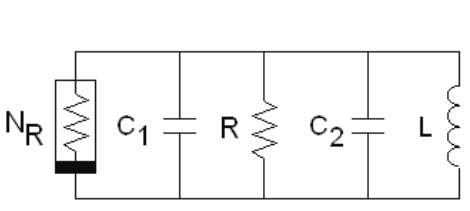
\includegraphics[width=0.9\textwidth]{Images/fig1(a).png}
		\caption{(a)}
		\label{fig:1a}
	\end{subfigure}%
	\begin{subfigure}[b]{0.5\textwidth}
		\centering
		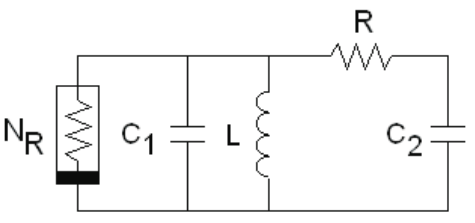
\includegraphics[width=0.9\textwidth]{Images/fig1(b).png}
		\caption{(b)}
		\label{fig:1b}
	\end{subfigure}
	% c and d
	\begin{subfigure}[b]{0.5\textwidth}
		\centering
		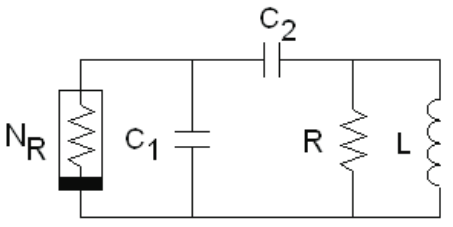
\includegraphics[width=0.9\textwidth]{Images/fig1(c).png}
		\caption{(c)}
		\label{fig:1c}
	\end{subfigure}%
	\begin{subfigure}[b]{0.5\textwidth}
		\centering
		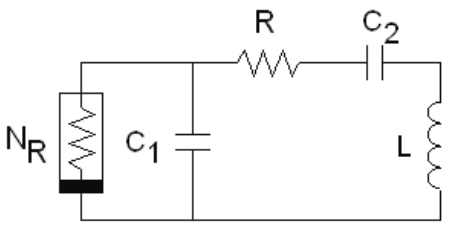
\includegraphics[width=0.9\textwidth]{Images/fig1(d).png}
		\caption{(d)}
		\label{fig:1d}
	\end{subfigure}
	% e and f
	\begin{subfigure}[b]{0.5\textwidth}
		\centering
		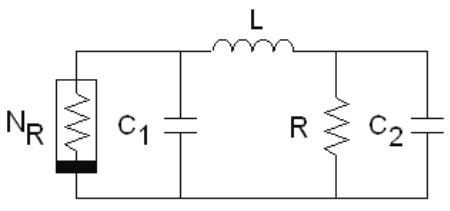
\includegraphics[width=0.9\textwidth]{Images/fig1(e).png}
		\caption{(e)}
		\label{fig:1e}
	\end{subfigure}%
	\begin{subfigure}[b]{0.5\textwidth}
		\centering
		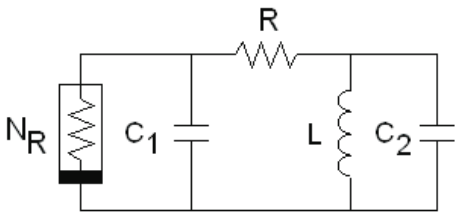
\includegraphics[width=0.9\textwidth]{Images/fig1(f).png}
		\caption{(f)}
		\label{fig:1f}
	\end{subfigure}
\end{figure}
\begin{figure}[H]
	\centering
	\caption{Fig 1. Possible configurations for circuit}
	% g and h
	\begin{subfigure}[b]{0.5\textwidth}
		\centering
		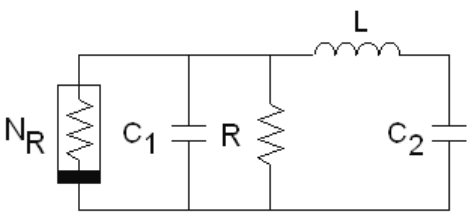
\includegraphics[width=0.9\textwidth]{Images/fig1(g).png}
		\caption{(g)}
		\label{fig:1g}
	\end{subfigure}%
	\begin{subfigure}[b]{0.5\textwidth}
		\centering
		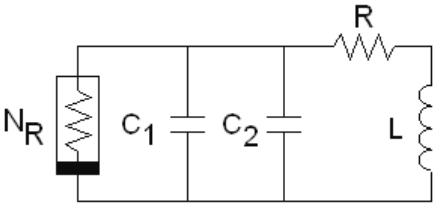
\includegraphics[width=0.9\textwidth]{Images/fig1(h).png}
		\caption{(h)}
		\label{fig:1h}
	\end{subfigure}
\end{figure}
Configuration (g) and (h) can be immediately rejected. \linebreak
In (g) the characteristic of resistance R can be absorbed in the characteristics of non-linear resistor $N_R$.
In (h) the $C_1$ and $C_2$ capacitances can be replaced by a single effective capacitor $C=C_1+C_2$. 
So in both of these configurations all circuit elements donot give unique contribution. Thus they can be rejected.\linebreak

For (a) and (b), the DC equilibrium calculations show that non-linear resistor gets short-circuited by the inductor. 
For (c) and (d), the DC equilibrium calculations show that non-linear resistor terminals are open.
So all the four configurations can be rejected. \linebreak

The remaining configuration (e) and (f) are both valid, but Chua selected configuration (f) because the RLC subcircuit generates oscillations.
%
%subsection 2.3
\subsection{Final Circuit}
The final Chua circuit is given as follows :
\begin{figure}[H]
	\centering
	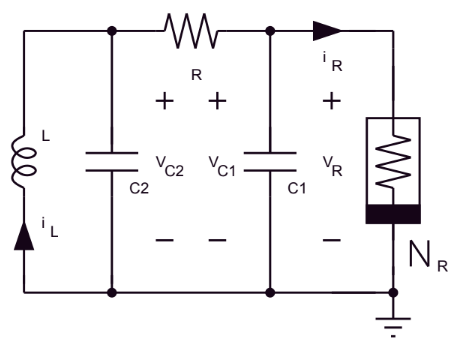
\includegraphics[width=0.6\textwidth]{Images/fig2_final.png}
	\caption{Fig 2. Chua's Circuit}
\end{figure}
%
%%%%%%%%%%%%%%%%%%%%%%%%%%%%%%%%%%%%%%%%%%%%%%%%%%%%%%%%%%%%
% SECTION 3 - STATE EQUATIONS AND SIMULATION
\section{State Equations and Simulations}
%subsection 3.1
\subsection{State Equations}
The equations of Chua's circuit are given as a system of three coupled differential equations :
\begin{align}
	C_1 \dfrac{dv_{C_1}}{dt}&=G\left( v_{C_2}-v_{C_1} \right)-g(v_{C_1}) \label{eq:1} \\
	C_2 \dfrac{dv_{C_2}}{dt}&=G\left( v_{C_1}-v_{C_2} \right)-i_L \label{eq:2}\\
	L \dfrac{i_L}{dt}&=-v_{C_2}\label{eq:3}
\end{align}
where, $G=\dfrac{1}{R}$ is the conductance, and $g(x)$ is a piece-wise linear function. It is given as :
\begin{align}
	g(v)&=m_0v+\dfrac{1}{2}(m_1-m_0)\left[ |v+B_p|-|v-B_p| \right] \label{eq:4}
\end{align}
where,
\begin{align*}
	m_0 &\implies \text{slope of outer region} \\
	m_1 &\implies \text{slope of inner region} \\
	B_P &\implies \text{breakpoints (both positive and negative values)}
\end{align*}
%
%subsection 3.2 - simulations
\subsection{Simulation}
The variables were redefined and all constants were taken to right hand side to make handling the equations easier.
\begin{align}
	\dfrac{dx}{dt}&=\dfrac{1}{C_1}\left\{ G\left( y-x \right)-g(x) \right\} \label{eq:5} \\
	\dfrac{dy}{dt}&=\dfrac{1}{C_2}\left\{ G\left( x-y \right)-z \right\} \label{eq:6} \\
	\dfrac{dz}{dt}&=-\dfrac{y}{L} \label{eq:7}
\end{align}
where,
\[ x \equiv v_{C_1} \quad y \equiv v_{C_2} \quad z \equiv i_L \]
The equation $g(x)$ remains the same as in (\myref{eq:4}).\linebreak
The equations are solved numerically using Runge Kutta 4 method in Python. All plots are made using Gnuplot.
%
%subsubsection 3.2.1 - Pyhton
\subsubsection{Python Codes}
The code for RK4 is as follows :
\lstinputlisting[language=Python]{/home/ashmita/Desktop/ASHMITA/APanda_Lib/chua_circuit_simulations.py}
The code inputs the three differential equations as a column vector F which is a function of x, y, z and t (time). x, y and z are arranged as column vector b. For the first iterations, it has the initial values. 
h is the increment factor. N is the number of iterations. $t_0$ is the initial time value. \linebreak

The `append.file()' function saves the data points (t, x, y and z) after each iteration in a file (filename provided to function as variable `name'). All codes for manipulation with files is as follows :
\lstinputlisting[language=Python]{/home/ashmita/Desktop/ASHMITA/APanda_Lib/handling_files.py}
%
% subsubsection 3.2.2 - plots with dimensionless constants
\subsubsection{Plots with Dimensionless Constants}
The following values were used for the constants :
\[ G=0.7 \quad C_1=1/9 \quad C_2=1 \quad L=1/7 \quad B_p=1 \quad m_0=-0.5 \quad m_1=-0.8 \]
The function g(v) in (\myref{eq:4}) can be plotted using the constants. 
\begin{figure}[H] %fig 3
	\centering
	\includegraphics[width=0.75\textwidth,height=0.3\textheight]{Plots/fig3_g(v).png}
	\caption{Fig 3. Three Segment Linear Function : g(v)}
\end{figure}
The code for defining the function, initial values and calling the function is :
\lstinputlisting[language=Python]{/home/ashmita/Desktop/ASHMITA/NISER Study/7th Semester/Open Lab/Non-Linear Circuit/Dimensionless/dimensionless_chua.py}
The data file obtained is plotted using Gnuplot.
\begin{figure}[H] % fig 4
	\centering
	\includegraphics[width=0.8\textwidth]{Plots/fig4_dimensionless_plot.png}
	\caption{Fig 4. 3D plot of $v_{C_1}$ vs $v_{C_2}$ for dimensionless constants}
\end{figure}
Thus, we do obtain a double scroll attractor for the Chua Circuit. In principle, the Chua Ciruit does exhibit chaotic behaviour. 
%
%subsubsection 3.2.3 - Varying R with dimensionful constants
\subsubsection{Varying R with Dimensionful Constants}
Now, we will attempt to use constants which represent actual dimensionful values and try to observe how the graph changes when we change the value of resistance $R$. \linebreak

We will define conversion factors to relate the value of our constants to values of actual electronic circuit components. Current will be measured in Amperes(A), potential differences in Volts(V), capacitances in Farads(F), inductance in Henry(H) and resistance in Ohm($\Omega$). Resistivity is expressed in Siemens(S)\linebreak
If we want currents of milliamperes to be in the circuit, we will adjust all current values by 1000. It will thus increase resistances and inductance by 1000, while decreasing capacitances by the same factor. Also, we can also rescale the values of time by some factor k in (\myref{eq:3}). This will leave all resistances unaffected, and all capacitors and inductors will be scaled by same factor k. For ease of using values in the code, I have chosen k to be $10^{-4}$, i.e., I rescale all capacitances and inductances by $10^{-4}$. This gives us the final conversion factors as :
\begin{align*}
	R & : 1 \equiv 1000 \Omega = 1k\Omega \\
	C_1, C_2 & : 1 \equiv 10^{-7} F = 100 nF \\
	L & : 1 \equiv 10^{-1} H = 100 mH \\
	m_0, m_1 & : 1 \equiv 10^{-3} S = 1 mS \\
	B_p & : 1 \equiv 1 V
\end{align*}
So, the constants used in the previous part correspond to :
\begin{equation*}
	R=1.43k\Omega \; ;  C_1=11.11 nF \; ; C_2=100 nF \; ; L=14.29 mH \; ; B_p = 1V \; ; m_0 = -0.5 mS \; ; m_1 = -0.8 mS
\end{equation*}
We will now attempt to vary R and observe how the output changes. \linebreak
The code for defining the function, initial values, varying R values and calling the function is :
\lstinputlisting[language=Python]{/home/ashmita/Desktop/ASHMITA/NISER Study/7th Semester/Open Lab/Non-Linear Circuit/Varying R/varying_R.py}
Plotting the data files obtained in Gnuplot. 
\begin{figure}[H] %fig 5
	\centering
	% a and b
	\caption{Fig 5. R Bifurcation in Theoretical Chua Circuit using a Three Segment Non-Linear Resistance}
	\begin{subfigure}[b]{0.5\textwidth}
		\centering
		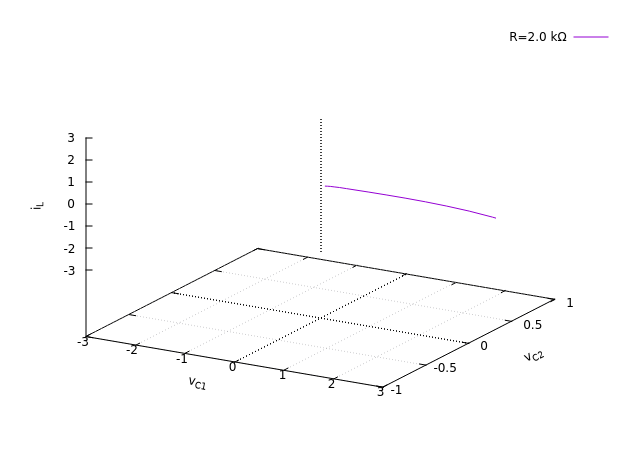
\includegraphics[width=\textwidth]{Plots/fig5(a)_2k.png}
		\caption{(a) $R=2.0k\Omega$}
	\end{subfigure}%
	\begin{subfigure}[b]{0.5\textwidth}
		\centering
		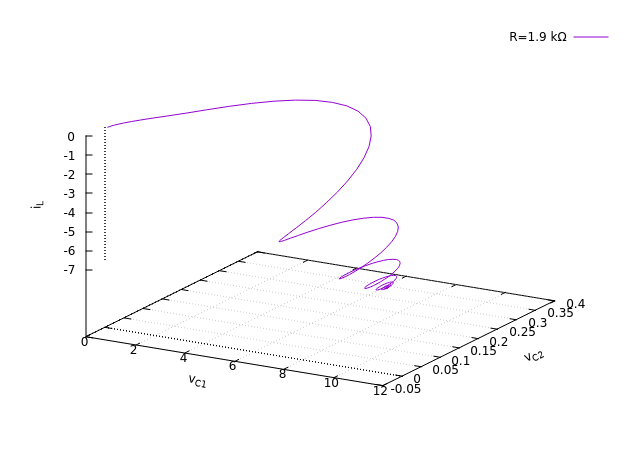
\includegraphics[width=\textwidth]{Plots/fig5(b)_1.9k.png}
		\caption{(b) $R=1.9k\Omega$}
	\end{subfigure}
\end{figure}
\begin{figure}[H] %fig 5 contd
	\centering
	% c and d
	\begin{subfigure}[b]{0.5\textwidth}
		\centering
		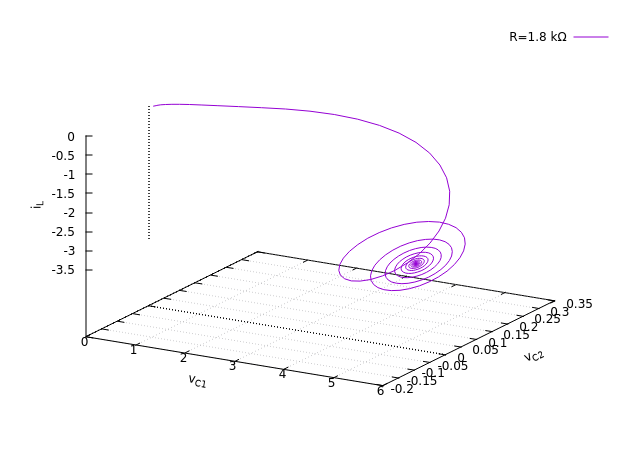
\includegraphics[width=\textwidth]{Plots/fig5(c)_1.8k.png}
		\caption{(c) $R=1.8k\Omega$}
	\end{subfigure}%
	\begin{subfigure}[b]{0.5\textwidth}
		\centering
		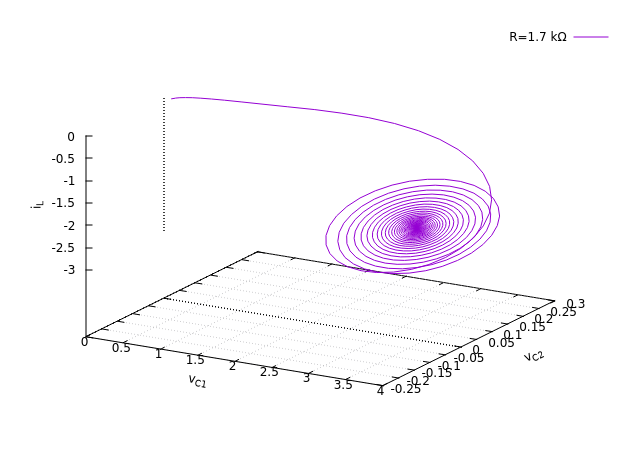
\includegraphics[width=\textwidth]{Plots/fig5(d)_1.7k.png}
		\caption{(d) $R=1.7k\Omega$}
	\end{subfigure}
	% e and f
	\begin{subfigure}[b]{0.5\textwidth}
		\centering
		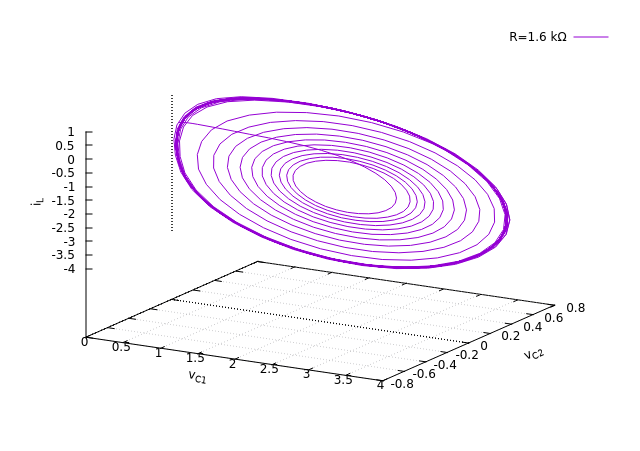
\includegraphics[width=\textwidth]{Plots/fig5(e)_1.6k.png}
		\caption{(e) $R=1.6k\Omega$}
	\end{subfigure}%
	\begin{subfigure}[b]{0.5\textwidth}
		\centering
		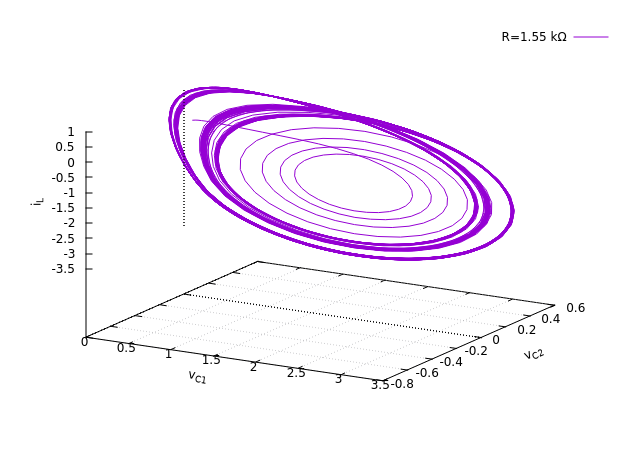
\includegraphics[width=\textwidth]{Plots/fig5(f)_1.55k.png}
		\caption{(f) $R=1.55k\Omega$}
	\end{subfigure}
	% g and h
	\begin{subfigure}[b]{0.5\textwidth}
		\centering
		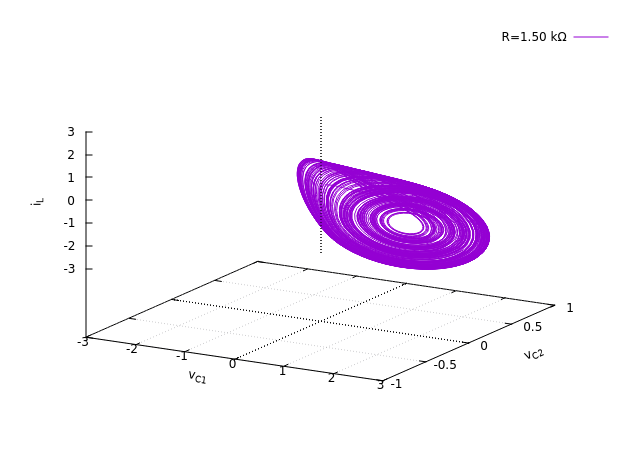
\includegraphics[width=\textwidth]{Plots/fig5(g)_1.5k.png}
		\caption{(g) $R=1.5k\Omega$}
	\end{subfigure}%
	\begin{subfigure}[b]{0.5\textwidth}
		\centering
		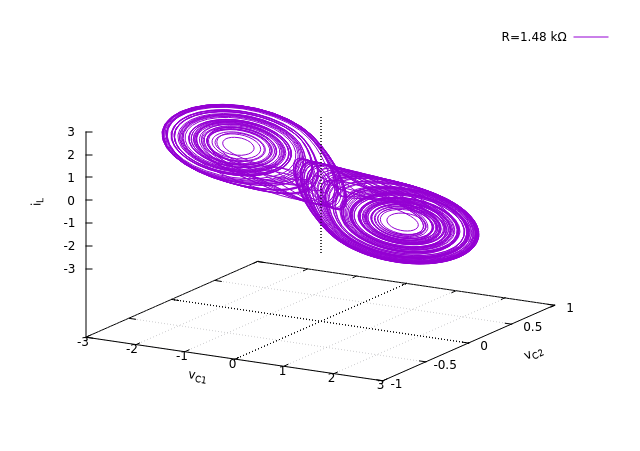
\includegraphics[width=\textwidth]{Plots/fig5(i)_1.48k.png}
		\caption{(h) $R=1.48k\Omega$}
	\end{subfigure}
	% i and j
	\begin{subfigure}[b]{0.5\textwidth}
		\centering
		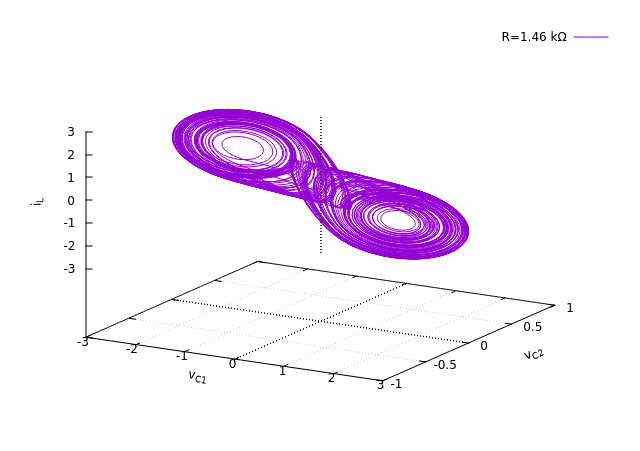
\includegraphics[width=\textwidth]{Plots/fig5(k)_1.46k.png}
		\caption{(i) $R=1.46k\Omega$}
	\end{subfigure}%
	\begin{subfigure}[b]{0.5\textwidth}
		\centering
		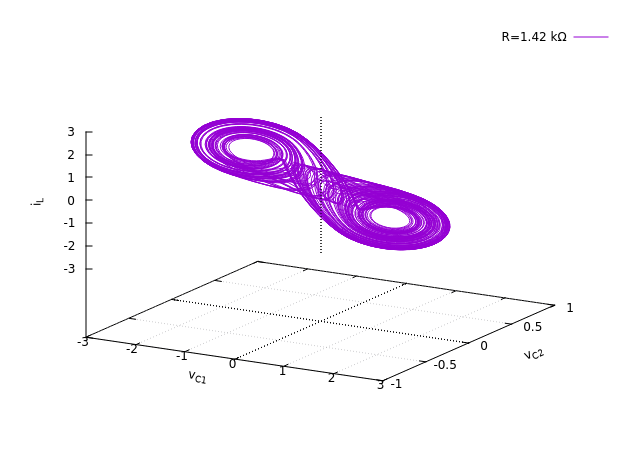
\includegraphics[width=\textwidth]{Plots/fig5(n)_1.42k.png}
		\caption{(j) $R=1.42k\Omega$}
	\end{subfigure}
\end{figure}
%
\begin{figure}[H] %fig 5 contd
	\centering
	% k and l
	\begin{subfigure}[b]{0.5\textwidth}
		\centering
		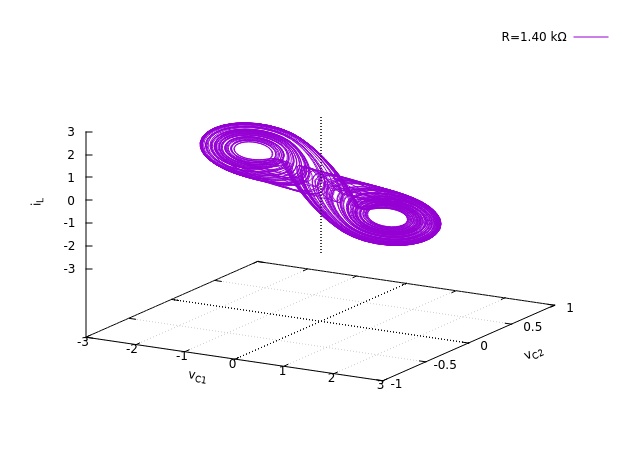
\includegraphics[width=\textwidth]{Plots/fig5(o)_1.40k.png}
		\caption{(k) $R=1.4k\Omega$}
	\end{subfigure}%
	\begin{subfigure}[b]{0.5\textwidth}
		\centering
		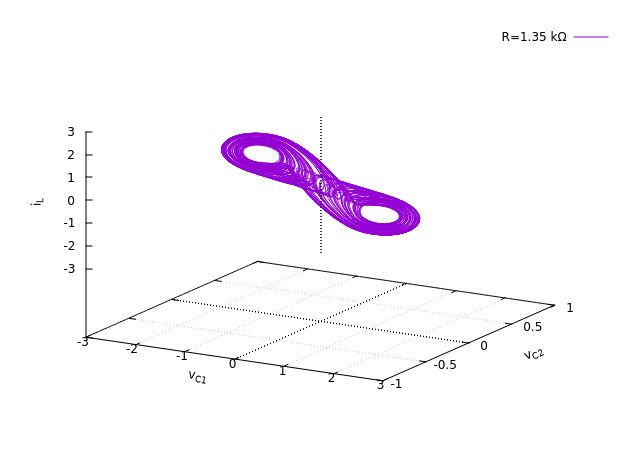
\includegraphics[width=\textwidth]{Plots/fig5(p)_1.35k.png}
		\caption{(l) $R=1.35k\Omega$}
	\end{subfigure}
	% m and n
	\begin{subfigure}[b]{0.5\textwidth}
		\centering
		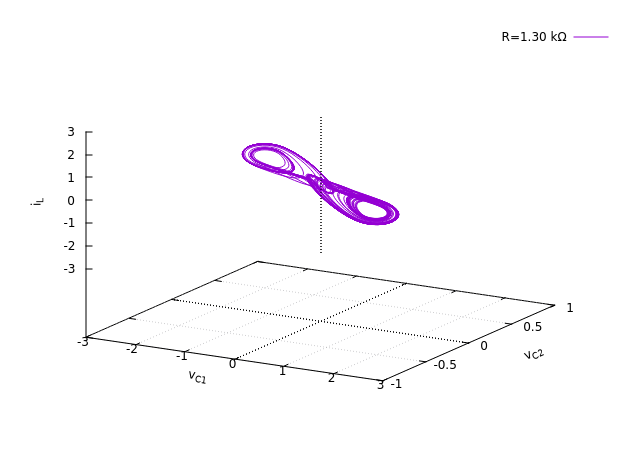
\includegraphics[width=\textwidth]{Plots/fig5(q)_1.30k.png}
		\caption{(m) $R=1.3k\Omega$}
	\end{subfigure}%
	\begin{subfigure}[b]{0.5\textwidth}
		\centering
		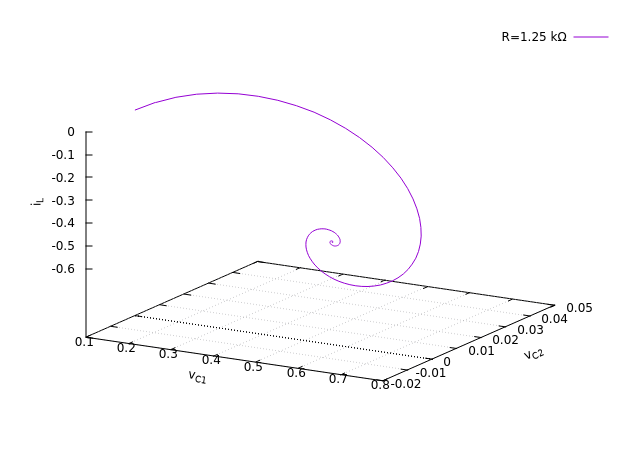
\includegraphics[width=\textwidth]{Plots/fig5(r)_1.25k.png}
		\caption{(n) $R=1.25k\Omega$}
	\end{subfigure}
	% o and p
	\begin{subfigure}[b]{0.5\textwidth}
		\centering
		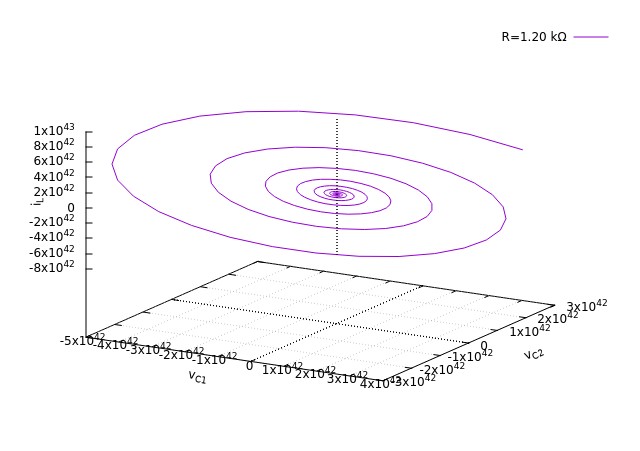
\includegraphics[width=\textwidth]{Plots/fig5(s)_1.20k.png}
		\caption{(o) $R=1.2k\Omega$}
	\end{subfigure}%
	\begin{subfigure}[b]{0.5\textwidth}
		\centering
		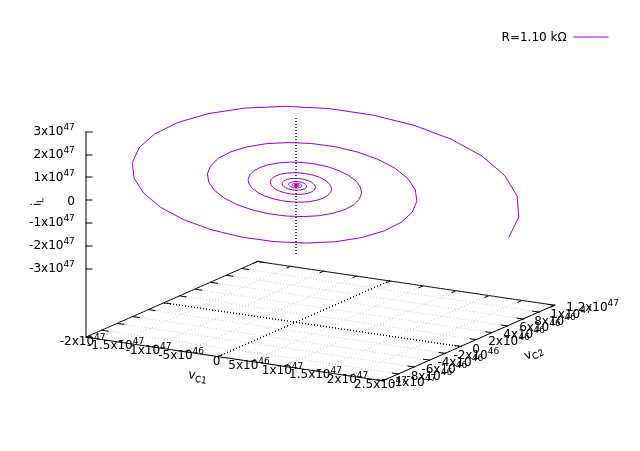
\includegraphics[width=\textwidth]{Plots/fig5(t)_1.10k.png}
		\caption{(p) $R=1.1k\Omega$}
	\end{subfigure}
\end{figure}
We observe that $R=2.0 k\Omega$ shows DC Equilibrium. As resistance is reduced, the characteristics looks like an unbounded spiral. \linebreak
The Rossler Attractor forms around $R=1.5 k\Omega$ and the Double Scroll Attractor is first formed at $R=1.48k\Omega$. As the resistance is further reduced, the size of the double scroll also decreases. \linebreak
By $R=1.25k\Omega$ the double scroll character is lost, and for lower resistances the graphs show a spiral with no upper bound. The values of $v_{C_1}$, $v_{C_2}$ and $i_L$ apparently take values in the ranges of $10^{43}$ and $10^{47}$. This is not physically possible.
%
%subsection 4 - Problems with Simulation
\subsection{Problems with Simulation}
The current simulation of the Chua Circuit is not physically viable, as is evident from the graphs obtained for various values of resistance. It predicts that except for a small window of resistance values (from $R=1.5k\Omega$ to $R=1.3k\Omega$) the values of voltages and current is not bounded. \linebreak

The problems arises because we have failed to take into account the fact that all physical resistors are eventually passive, i.e., for large enough values of voltages applied across its terminals, the power consumed by the resistor becomes positive. \linebreak
In our current equation (\myref{eq:4}) and graph of g(v), we see that the condition of eventual passivisity has not been taken into account. The power consumed by the resistor is negative for all values of voltages.
%%%%%%%%%%%%%%%%%%%%%%%%%%%%%%%%%%%%%%%%%%%%%%%%%%%%%%%%%%
%section 4 - Simulation to Practical Design
\section{Simulation to Practical Design}
%%
%subsection 4.1 - Negative Resistance
\subsection{Negative Resistance}
To implement a Chua Circuit practically we first need to construct a negative resistance which follows the characteristics of $g(v)$ graph. One way to construct a negative resistance is to connect three positive linear resistors to a voltage controlled voltage source (VCVS).
%
%subsubsection 4.1.1-VCVS
\subsubsection{Voltage Controlled Voltage Source}
A VCVS is defined to be an ideal circuit element with two input and two output terminals such that no current flows between the input terminals and voltage across output terminals is dependent on the volatge across input terminals.
\[ v_o= f(v_d) \]
$f(.)$ could have any functional dependence, but the simplest non-trivial relation occurs when it is linear. 
\begin{figure}[H]
	\centering
	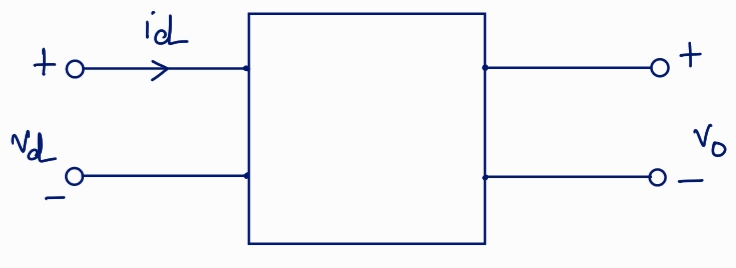
\includegraphics[width=0.7\textwidth]{Images/fig6_vcvs.png}
	\caption{Fig 6. Voltage Controlled Voltage Source}
\end{figure} 
%
%subsubsection 4.1.2 - negative resistance using VCVS
\subsubsection{Negative Resistance using ideal VCVS}
The circuit diagram to build a negative resistance using an ideal VCVS and three linear resistors is given as follows :
\begin{figure}[H]
	\centering
	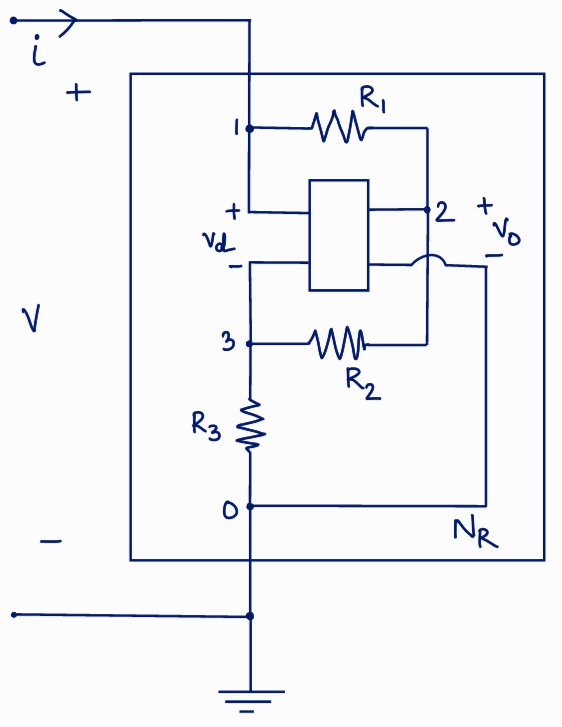
\includegraphics[width=0.5\textwidth]{Images/fig7_Nr with vcvs.png}
	\caption{Fig 7. Negative Resistance using VCVS}
\end{figure}
Let us assume the VCVS follows a linear relationship :
\begin{equation}
	v_o=Av_d \label{eq:8}
\end{equation}
A is some proportionality constant. \linebreak

Now, Kirchoff's Current Law (KCL) says that \textit{for any node in an electrical circuit, the sum of the currents entering the node is equal to the sum of the currents leaving the node}. \linebreak

Applying KCl on node (1) (in Fig 7):
\begin{equation}
	i=i_1 \quad ; \quad  i_1=\dfrac{v-v_o}{R_1} \label{eq:9}
\end{equation}
We can write this because no current goes inside VCVS.\linebreak

Now, Kirchoff's Voltage Law (KVL) says that \textit{if we move around a closed loop in a fixed direction then the sum of all the potential differences around the loop is zero.} \linebreak

Applying KVL along loop 1-2-3-0 (in Fig 7):
\begin{align}
	v&=v_d + i_3R_3 \label{eq:10} \\
	i_3&=\dfrac{v_o}{R_2+R_3} \label{eq:11}
\end{align}
Using (\myref{eq:11}) in (\myref{eq:10}) :
\begin{align}
	v&=v_d + \dfrac{v R_3 v_d}{R_2+R_3} = \dfrac{R_2+(1+A)R_3}{R_2+R_3}v_d \nonumber \\
	\intertext{Now, using (\myref{eq:8}) in the above equation : }
	\therefore v&= \left\{ \dfrac{R_2+(1+A)R_3}{A(R_2+R_3)} \right\}v_o \label{eq:12}
\end{align}
We can now calculate the current $i$ using (\myref{eq:9}) :
\begin{align*}
	i&=\dfrac{v}{R_1}-\dfrac{v_o}{R_1} \\
	\intertext{Using equation of $v$ and $v_o$ (\myref{eq:12}) :}
	\implies i &= \dfrac{v}{R_1}-\dfrac{1}{R_1}\left\{ \dfrac{A(R_2+R_3)}{R_2+(1+A)R_3}v \right\} \\
	\implies i &= \dfrac{vR_2+vR_3+vAR_3-AR_2v-AR_3v}{R_1\left[ R_2+(1+A)R_3 \right]}
\end{align*}
So we finally obtain :
\begin{equation}
	\therefore i = \left\{ \dfrac{R_2(1-A)+R_3}{R_1\left[ R_2+(1+A)R_3 \right] } \right\} \label{eq:13}
\end{equation}
Now if we take A to be very large, $A\gg 1$, greater than $R_1, R_2$ and $R_3$, we can write :
\begin{align*}
	\implies i & \thickapprox \dfrac{-R_2A+R_3}{R_1(R_2+R_3A)}v \\
	\intertext{Also, as $R_2A \gg R_3$ and $R_1R_3A \gg R_1R_2$ :}
	\implies i & \thickapprox -\dfrac{R_2A}{R_1R_3A}v \thickapprox -\dfrac{R_2}{R_1R_3}v
\end{align*}
We can now set $R_1=R_2$, and we obtain :
\begin{equation}
	i=-\dfrac{1}{R_3}v \label{eq:14}
\end{equation}
Thus it now appears that the segment $N_R$ (in Fig 7) now has negative resistance $-R_3$. 
%
%subsubsecrion 4.1.3 - opamps as VCVS
\subsubsection{Op-Amps as VCVS}
An opamp is the practical or real-life approximation of a VCVS. The voltage applied across inverting and non-inverting terminals produces voltage at output terminal, if we take the reference terminal to be ground.
\begin{figure}[H]
	\centering
	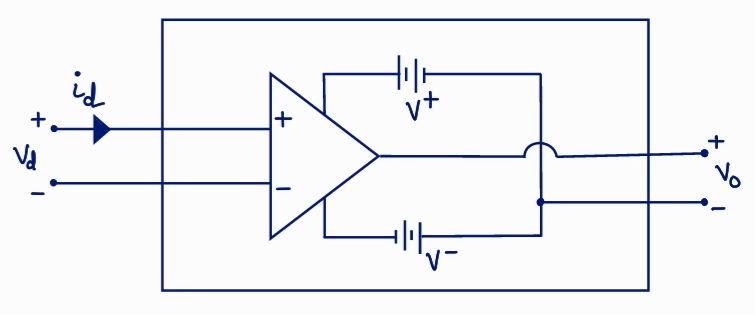
\includegraphics[width=0.6\textwidth]{Images/fig8_opamp as vcvs.png}
	\caption{Fig 8. Op-amp as VCVS}
\end{figure}
Ideal opamps there is no current entering the circuit, i.e., $i_d=0$ and the loop gain is infinite. But typically, most opamps produce output voltages 100,000 times larger than the potential difference between input terminals. \linebreak

The output of a opamp becomes constant at some values of $v_d=\pm E_{sat}$.
\begin{align*}
	\text{For } v_d\geq \dfrac{E_{sat}}{A}+v_{OS} & \quad \text{: positive saturation region} \\
	\text{For } v_d\leq-\dfrac{E_{sat}}{A}+v_{OS} & \quad \text{: negative saturation region} \\
	\text{For } -\dfrac{E_{sat}}{A}+v_{OS}< v_d < \dfrac{E_{sat}}{A}+v_{OS} & \quad \text{: linear region}
\end{align*}
$v_{OS}$ is the offset voltage. 
\begin{figure}[H]
	\centering
	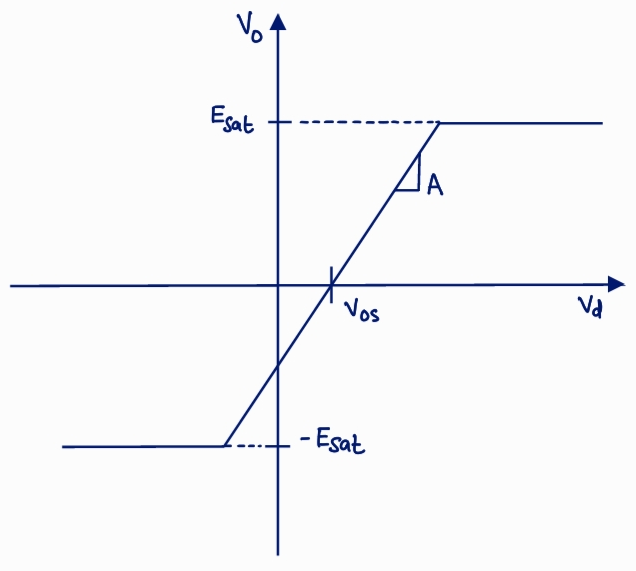
\includegraphics[width=0.5\textwidth]{Images/fig9_opamp characteristics.png}
	\caption{Fig 9. Output Characteristics of an Op-Amp}
\end{figure}
From here on, we will assume :
\[ v_{OS} =0 \quad ; \quad i_d=0 \quad ; \quad v_o=f(v_d) \]
%
%subsubsection 4.1.4
\subsubsection{Negative Resistance using Op-Amps}
We can build a negative resistance using the analysis we did previously, while using Op-Amp as VCVS.
\begin{figure}[H]
	\centering
	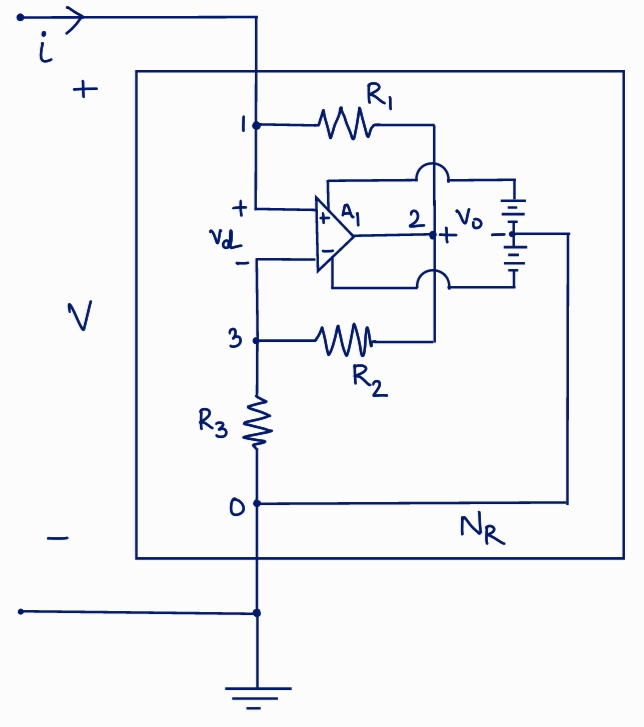
\includegraphics[width=0.5\textwidth]{Images/fig10_negative resistance using opamp.png}
	\caption{Fig 10. Negative Resistance using Op-Amps}
\end{figure}
From previous circuit analysis we have :
\begin{equation}
	i=\dfrac{v-v_o}{R_1} \quad ; \quad v=v_d+\dfrac{R_3}{R_2+R_3}v_o \quad ; \quad v_o = Av_d \label{eq:15}
\end{equation}
As now we have an op-amp, there are three distinct regions depending on the voltage behavior :
\begin{align*}
	\text{Negative Saturation} & : \qquad  v_o = -E_{sat} \qquad ; \qquad v_d \leq -\dfrac{E_{sat}}{A} \\
	\text{Linear Region} & : \qquad  v_o=Av_d \qquad ; \qquad -\dfrac{E_{sat}}{A} < v_d < \dfrac{E_{sat}}{A} \\
	\text{Positive Saturation} & : \qquad v_0=E_{sat} \qquad ; \qquad v_d\geq \dfrac{E_{sat}}{A} \\
\end{align*}
\textbf{\uline{Positive Saturation}} \linebreak %positive saturration
In the positive saturation region the output voltage is fixed at $E_{sat}$, even if the input changes.
\begin{equation}
	v_o = E_{sat} \qquad ; \qquad v_d \geq \dfrac{E_{sat}}{A} \label{eq:16}
\end{equation}
From (\myref{eq:15}) and (\myref{eq:16}), we have equation of current as :
\begin{equation}
	i=\dfrac{v}{R_1}-\dfrac{E_{sat}}{R_1} \label{eq:17}
\end{equation}
We can write the equation for voltage as :
\begin{align*}
	v&= v_d+\dfrac{R_3}{R_2+R_3}v_o \\
	\implies v & \geq \dfrac{E_{sat}}{A}+\dfrac{R_3}{R_2+R_3}E_{sat} \\
	\implies v & \geq E_{sat}\left\{ \dfrac{R_2+R_3+AR_3}{A(R_2+R_3)} \right\}
\end{align*}
So we finally obtain :
\begin{equation}
	v \geq \left\{ \dfrac{R_2+(1+A)R_3}{A(R_2+R_3)} \right\} E_{sat} \label{eq:18}
\end{equation}
So the minimum value of valid $v$ for positive saturation, or the positive breakpoint is given as :
\begin{equation}
	B^+_P = \dfrac{R_2+(1+A)R_3}{A(R_2+R_3)} E_{sat} \label{eq:19}
\end{equation}
Now if A is very large, we have $(1+A)R_3+R_2 \longrightarrow AR_3$. So we obtain the breakpoint as :
\begin{equation}
	B^+_P \simeq \dfrac{R_3}{R_2+R_3}E_{sat} \label{eq:20}
\end{equation}
Slope of the graph is given as :
\begin{equation}
	m_o=\dfrac{1}{R_1} \label{eq:21}
\end{equation}
\textbf{\uline{Negative Saturation}} \linebreak %negative saturation
In negative saturation, $v_o=-E_{sat}$. As all other equations remain same, we have the breakspoint as :
\begin{equation}
	B^-_P = - \dfrac{R_2+(1+A)R_3}{A(R_2+R_3)}E_{sat} \label{eq:22}
\end{equation}
For very large A, we get the breakpoint as :
\begin{equation}
	B^-_P \simeq -\dfrac{R_3}{R_2+R_3}E_{sat} \label{eq:23}
\end{equation}
The slope is still $m_o$. \linebreak
\textbf{\uline{Linear Region}} \linebreak %linear region
In the linear region, we have the standard circuit analysis we did before given in (\myref{eq:15}). \linebreak
Writing voltage $v_d$ in terms of $v$ :
\begin{align*}
	v&=v_d+\dfrac{R_3}{R_2+R_3}v_o \\
	\implies v &= v_d+\dfrac{R_3}{R_2+R_3}Av_d \\
	\implies v&= \dfrac{R_2+(1+A)}{R_2+R_3} v_d 
\end{align*}
Therefore, we obtain :
\begin{equation}
	v_d= \dfrac{R_2+R_3}{R_2+(1+A)R_3}v \label{eq:24}
\end{equation}
Using this (\myref{eq:24}) to find current $i$ :
\begin{equation}
	i = \dfrac{(1-A)R_2+R_3}{R_1\left[ R_2+(1+A)R_3 \right]}v \label{eq:25}
\end{equation}
For large A, we have :
\begin{equation}
	i \simeq - \dfrac{R_2}{R_1R_3}v \label{eq:26}
\end{equation}
The linear region is characterised by :
\begin{align*}
	& -\dfrac{E_{sat}}{A}<v_d<\dfrac{E_{sat}}{A} \\
	\implies & -\dfrac{E_{sat}}{A}<\dfrac{R_2+R_3}{R_2+(1+A)R_3}v < \dfrac{E_{sat}}{A} \\
	\intertext{For $v$ : }
	\therefore & -E_{sat}\dfrac{R_2+(1+A)R_3}{A(R_2+R_3)} < v < E_{sat} \dfrac{R_2+(1+A)R_3}{A(R_2+R_3)} \\
	\intertext{For large A, we have :}
	\implies & -E_{sat}\dfrac{R_3}{R_2+R_3}<v<E_{sat}\dfrac{R_3}{R_2+R_3} \\
	\intertext{From (\myref{eq:20}) and (\myref{eq:23}) :}
	\therefore & B^-_P < v < B^+_P 
\end{align*}
Thus, when voltage $v$ lies between breakpoints, the op-amp functions in the linear region. \linebreak
Slope of the I-V graph in this region is :
\begin{equation}
	m_1=-\dfrac{R_2}{R_1R_3} \label{eq:27}
\end{equation}
The I-V characteristics of negative resistance implemented using op-amps should be of the form :
\begin{figure}[H]
	\centering
	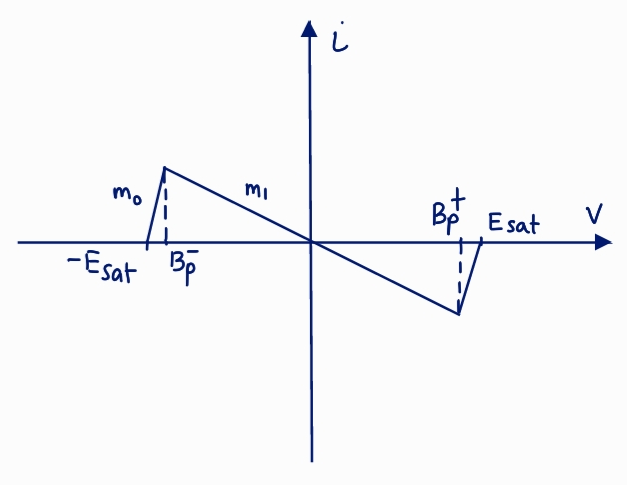
\includegraphics[width=0.5\textwidth]{Images/fig11_negative characteristics.png}
	\caption{Fig 11. Expected I-V Characteristics of Negative Resistance}
\end{figure}
%%
%subsection 4.2 - Non-Linear Resistance
\subsection{Non-Linear Resistance}
Now that we have the negative resistances, we would like to implement our Non-Linear resistance to be used in the circuit. To do so, we need to put two negative resistances in parallel. \linebreak
$N_{R_1}$ includes resistances $R_1$, $R_2$ and $R_3$. It has slopes $m_{01}$, $m_{11}$ and breakpoints $\pm B_{P1}$. \linebreak
$N_{R_2}$ includes resistances $R_4$, $R_5$ and $R_6$. It has slopes $m_{02}$, $m_{12}$ and breakpoints $\pm B_{P2}$. \linebreak

We will assume $R_1=R_2$ and $R_4=R_5$. 
\begin{figure}[H]
	\centering
	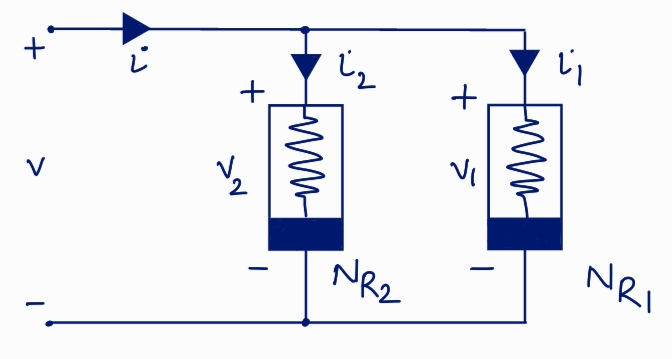
\includegraphics[width=0.6\textwidth]{Images/fig12_nonlinear.png}
	\caption{Fig 12. Non-linear Resistance}
\end{figure}
So for $N_{R_1}$ we have :
\begin{equation}
	m_{01}=\dfrac{1}{R_1} \qquad ; \qquad m_{11}=-\dfrac{1}{R_3} \qquad ; \qquad B_{P1}=\pm \dfrac{R_3}{R_2+R_3}E_{sat} \label{eq:28}
\end{equation}
For $N_{R_2}$ we have :
\begin{equation}
	m_{02}=\dfrac{1}{R_4} \qquad ; \qquad m_{12}= -\dfrac{1}{R_6} \qquad ; \qquad B_{P2}= \pm \dfrac{R_6}{R_5+R_6}E_{sat} \label{eq:29} 
\end{equation}
Slopes of $N_{R_1}$ and $N_{R_2}$ are connected to the slopes of the combined graph is :
\begin{equation}
	m_{11}+m_{02}=m_0 \qquad ; \qquad m_{11}+m_{12}=m_1 \label{eq:30}
\end{equation}
The expected I-V graph of non-linear resistance is as follows :
\begin{figure}[H]
	\centering
	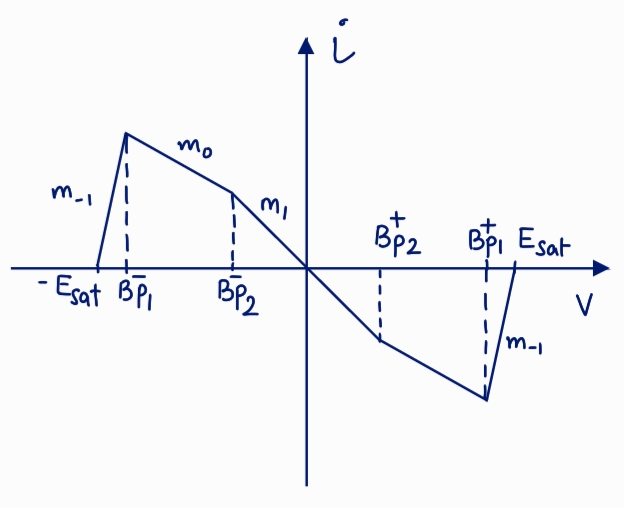
\includegraphics[width=0.6\textwidth]{Images/fig13_nonlinear characteristics.png}
	\caption{Fig 13. Expected I-V Characteristics of non-linear resistance}
\end{figure}
%%%%%%%%%%%%%%%%%%%%%%%%%%%%%%%%%%%%%%%%%%%%%%%%%%%%%%
%section 5 - Practical Implementation using LTSpice
\section{Practical Implementation with LTSpice}
LTSpice was used to practically implement the Chua Ciruit. The circuit design is used from the paper by Kennedy[{\color{red}{put ref}}] (Fig 101. \linebreak

All op-amps used are TL082, which was downloaded as a third-party tool from the website \url{http://www.chaotic-circuits.com/simulating-electronic-circuits/} and implemented into the circuit.\linebreak
%%
%subsection 5.1 - Component Values
\subsection{Setting Component Values}
9V voltage sources were used to power the op-amps. The values of resistances, capacitors and inductors used to implement the circuit is as follows :
\begin{align*}
	\intertext{\textbf{For $\bm{N_{R_1}}$ :}}
	R_1 &= 220\Omega \pm 5\% \\
	R_2 &= 220\Omega \pm 5\% \\
	R_3 &= 2.2k\Omega \pm 5\% \\
	\intertext{\textbf{For $\bm{N_{R_2}}$ :}}
	R_4 &= 22k\Omega \pm 5\% \\
	R_5 &= 22k\Omega \pm 5\% \\
	R_6 &= 3.3k\Omega \pm 5\% \\ 
	\intertext{\textbf{Rest of the circuit elements :}}
	C_1 &= 10nF \pm 5\% \\
	C_2 &= 100nF \pm 5\% \\
	L &= 18mH \pm 10\% \\
	R &= 2.0k\Omega \text{ to } 1.2k\Omega 
\end{align*}
$R$ is varied from $2.0k\Omega$ to $1.2k\Omega$ to observe the various stages of the bifurcation sequence. 
%%
%subsection 5.2 - Negative Resistance
\subsection{Negative Resistances}
First the negative resistances are individually implemented in LTSpice to ensure they function as we theoretically expect them to. The saturation voltage ($E_{sat}$) for TL082 and breakpoints for both resistors is also obtained. \linebreak

To measure the output voltage, a small resistance of value $R=10\Omega$ is put in series and the current across is plotted vs the input voltage.
%
%subsubsection 5.2.1 - N_{R_1}
\subsubsection{N\textsubscript{R1}}

The values of slopes for $N_{R_1}$ are obtained from (\myref{eq:28}) as :
\begin{align*}
	m_{01}&=4.545\times 10^{-3} S = 4.545 mS \\ 
	m_{11}&= -4.545\times 10^{-4} S = -0.4545 mS 
\end{align*}
The values of sloped for $N_{R_2}$ are obtained from (\myref{eq:29}) as :
\begin{align*}
	m_{02}&=4.545\times 10^{-5}S = 0.04545 mS \\
	m_{12}&=-0.303\times 10^{-3}S = -0.303 mS
\end{align*}
So the value of sloped for the 







\end{document}